\chapter{Modeling and Controller Design for the TU/e \texorpdfstring{$1$}{1}-DoF System}
\label{chap:application}




Consider the constant multiplier case given in \cite{carsten2} without proof. 

\begin{lem}Let $Q$ be a nonsingular symmetric matrix and $\mathcal{S}$ a subspace (and $S\in\mathbb{R}^{n\times s}$ is being a basis 
of $\mathcal{S}$) with $\zeta(S^TQS) = 0$. Then, $\inertia(S^TQS)+\inertia(S_\perp^T\inv{Q}S_\perp) = \inertia(Q)$.
\end{lem} 


\begin{proof} Consider the following simple quadratic form,
\[
\pmatr{1\\0}^T\pmatr{0 &1\\1 &0}\pmatr{1\\0} = 0
\]
although the multiplier is invertible. The extra hypothesis $\zeta(S^TQS) = 0$  avoids such situations. Assume, $\inertia(Q)=\{p,0,n\}$
Consider the following
\begin{align}
\inertia \left(\pmatr{S^T\\I}Q\pmatr{S&I}\right) &= \inertia\pmatr{0 &0\\0&Q} = \{p,s,n\}\\
&= \inertia \pmatr{S^TQS &0\\0&Q - QS\inv{(S^TQS)}S^TQ}\\
&= \inertia \pmatr{S^TQS &0\\0&\inv{Q} - S\inv{(S^TQS)}S^T} = \{p,s,n\}\\
& \Longrightarrow \inertia\pmatr{S^TQS &0\\0&S_\perp^T\inv{Q}S_\perp} = \{p,0,n\} = \inertia(Q)
\end{align}
where we used the fact that 
\[
x^T\inv{Q}x = x^TS\inv{(S^TQS)}S^Tx
\]
can only be satisfied if $x$ has a nonzero component in the image of $S$, since $\text{ker}(Q)=\{0\}$. Hence, zero inertia is removed by $S_\perp$. 
\end{proof}




\section{Human as Uncertain Filter}

As we have touched upon in \Cref{chap:litsurvey}, one can see the human action as a force input filtered through the
arm dynamics. Before we start deriving the relevant models, a few remarks seems proper to state here. 

As we have argued up to this point, passivity assumption on the human dynamics seems artificial, conservative and also
the evidence that is brought up for justification for it is questionable. Therefore, we would like to change the human
model or the source termination of the port with a refined impedance model, however, we have no substitute for such change. 

This might seem awkward to state, especially after putting so much emphasis on this issue. 











But, we have also scanned the neuroscience articles and seen that there is no consensus on how the human arm dynamics are altered. 
There are many studies with extraordinarily bold titles (which might be standard of publishing in the most prestigious journals),
but, in the end they still seem disagreeing with each other if not contradicting thus the results are unlike the titles are suggestive 
but not conclusive. \footnote{As an orthogonal comment to the beginners of the field, the scientific standard for claiming to have 
a solution is much different in the neuroscience than the engineering customs. The main problem is that most of these studies first 
define a hypothesis and then look for patterns to verify the behavior. However, another similar article uses almost the same 
experimental setup and reaches to a completely different set of conclusions. Many seem to suffer from the causality often described 
with \emph{All apples are red, this is red, therefore it is an apple}.}.







\section{Model Setup}
We present two possibilities of human modeling. In the first one, the uncertain human arm is taken from literature and 
in the second we just present the complexity of a possible (Quasi)-LPV model. 
\subsection{Uncertain LTI Model}
The synthesis problem that we want attack requires a human model together with the local/remote 
devices. We will delay the environment discussion until the next section. Our framework can be 
shown pictorially in \Cref{fig:genframe}. Here we assume that the human is watching a screen that
shows the remote environment or building up a virtual state of the environment by just interpreting
the force cues that s/he receives. For simplicity , we concentrate on the former case.

The most important difference with the current literature is that we skip the modeling the environment
and include its effect with an external perturbation denoted by $f_e$. As an example, a hard contact 
is modeled as a force perturbation at some point in time, restricting the position of the remote 
device. However, there are important relations that is being ignored such as the frequency spectrum
of the force signal $f_e$ is directly related to the position reference supplied by human $x_d$, and 
the resulting force input. As an advantage, this allows us to include active environments such as 
underwater current affecting the remote device in a deep-sea exploration mission etc. hence the environment 
need not to be passive at all. Instead, backdrivability is explicitly considered. The various mesurements
can be defined depending on what sort of a controller type is required. A typical selection is the position
and the force signals of remote and local site. 


\subsubsection{Assumptions}
\begin{itemize}
	\item We assume that the frequency content of the human reference generated by $f(vision)$ has no significant content
	at high frequencies. For this, we can introduce yet another low-pass filter or modify the existing $W_t$. 
	\item Similarly we assume that the frequency content of $f_e$ is dominant in the low-frequency band. 
	\item For now, we don't place transmission delays unilaterally or bilaterally around $K$ block. This would denote the
	local or remote device distance from the control station. It can be at the local or the remote site or even in between
	distant to both stations.
\end{itemize}
\begin{figure}%
\centering
\begin{tikzpicture}[>=stealth]
\node [draw,circle,inner sep=2pt] (junc) at (-3cm,0) {};
\node [draw] at (-4.2cm,0cm) (H) {$H_u(\Delta)$};
\node [draw] (K) at (-1.5,-1) {K};
\node [draw] (Hp) at (-1.5,0) {$H_p$};
\node [draw,outer sep=0] (mr1) at (1,0) {$M_{r1}$};
\node [draw] (mr2) at (3,0) {$M_{r2}$};
\node [draw] (brain) at (-4,2) {$f(vision)$};
\draw[<-] (junc.south) node[below right] {$-$}|- (K.west) node[below,midway] {$\tau_l$};
\draw[<-] (H.west) -- ++(-0.5,0) node[above left] {$x_d$} -| ++(-0.5,2) -- (brain.west);
\draw[->] (H.east) -- (junc.west);
\draw[->] (junc.east) -- (Hp.west);
\fill [pattern = north east lines] (mr1.south west) rectangle ([yshift=-2mm]mr2.south east);
\draw[decorate,decoration={zigzag,pre length=0.2cm,post length=0.2cm,segment length=6}] (mr1.20) -- (mr2.160);
\draw[decoration={markings,  
  mark connection node=dmp,
  mark=at position 0.5 with 
  {
    \node (dmp) [inner sep=0pt,transform shape,rotate=-90,minimum width=5pt,minimum height=1.5pt,draw=none] {};
    \draw ($(dmp.north east)+(2pt,0)$) -- (dmp.south east) -- (dmp.south west) -- ($(dmp.north west)+(2pt,0)$);
    \draw ($(dmp.north)+(0,-2.5pt)$) -- ($(dmp.north)+(0,2.5pt)$);
  }
}, decorate] (mr1.-15) -- (mr2.-165);
\draw[->] (K.east) -| ([xshift=-5mm]mr1.west) node[midway,below] {$\tau_r$}-- (mr1.west);
\draw[<-] (mr2.east) -- ++(5mm,0) node[right] {$f_e$};
\draw[->] (Hp.east) -- ++(5mm,0) node[right] (xl){$x_l$};
\draw[dashed,->] (mr2.north) |- ([yshift=1mm]brain.east);
\draw[dashed,->] (xl.north) |- ([yshift=-1mm]brain.east);
\draw[<-] (K.south) -- ++(0,-5mm) node[text width=3.5cm,below,align=center] {Various \\ Measurements};
\end{tikzpicture}
\caption{The general framework}%
\label{fig:genframe}%
\end{figure}



The inclusion of a human model as such allows us to model the hand tremor of a human with varying abilities. This is certainly 
important in rehabilitation problems where the individual has difficulty in maintaining a firm hand/arm position. In other words, 
for the same position reference input, different $H_{arm}$ models can lead to the hand tremor via some underdamped vibrational 
modes. In our particular example, we refer to an identified model found in the literature. 


We start with the identified model \cite{fucavus} : The basic block diagram is given in \Cref{fig:identifiedmodel}. The signal relations can be written as
\[
\pmatr{q\\x} = \bmatr{0 &W_{unc}\\H_{arm} & H_{arm}}\pmatr{p\\f}.
\]
The numerical data is given as (\cite{fucavus})
\[
H_{arm} =     \frac{0.1092 s^2 + 7.035 s + 329.5}{s^3 + 92.77 s^2 + 1921 s + 1.788e004}
\]
and 
\[
W_{unc}= 10^{th} \ \ order \ \ proper TF\text{ (large text to-be-replaced-later)}.%1.2252 \frac{(s^2 + 3.718s + 10.91) (s^2 + 71.58s + 1324) (s^2 + 16.27s + 242.3) (s^2 + 77.18s + 1948) (s^2 + 5.724s + 2285)}{%
%(s^2 + 3.07s + 5.277) (s^2 + 138.3s + 4795) (s^2 + 10.95s + 178.5) (s^2 + 30.16s + 1434) (s^2 + 8.164s + 2356)}
\]


\begin{figure}%
\centering
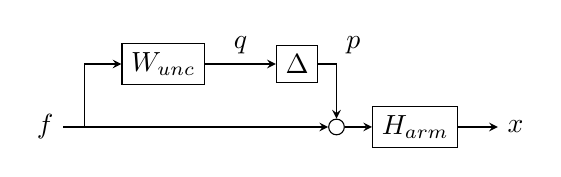
\begin{tikzpicture}[>=stealth]
\node at (-3.5cm,0) (f) {$f$};
\node [draw,circle,inner sep=2pt] (junc) at (0.2cm,0) {};
\node [draw] at (-2cm,0.8cm) (W) {$W_{unc}$};
\node [draw] at (-0.3cm,0.8cm) (delt) {$\Delta$};
\node [draw] at (1.2cm,0cm) (H) {$H_{arm}$};
\draw[->] (f) -- (junc.west);
\draw[->] (f) -- ++ (5mm,0) |- (W.west);
\draw[->] (W.east) -- (delt.west) node[midway,above] {$q$};
\draw[->] (delt.east) -| (junc.north) node[midway,above right] {$p$};
\draw[->] (junc.east) -- (H.west);
\draw[->] (H.east) -- ++(5mm,0) node[right] {$x$};
\end{tikzpicture}
\caption{The experimentally identified human model from \cite{fucavus}}%
\label{fig:identifiedmodel}%
\end{figure}

For our purposes we obtain a mapping from position to force via a partial inversion on the second channel. 
\[
\pmatr{q\\f} = \bmatr{-W_{unc} &W_{unc}\inv{H_{arm}}\\-1 &\inv{H_{arm}}}\pmatr{p\\x} = \bmatr{W_{unc}\\1}\bmatr{-1 &\inv{H_{arm}}}\pmatr{p\\x}
\]


\begin{figure}%
\centering

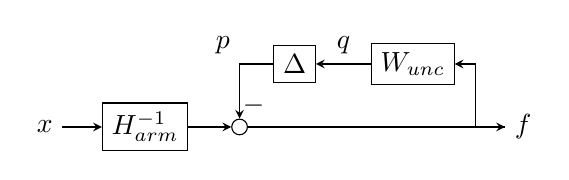
\begin{tikzpicture}[>=stealth]
\node at (0.6cm,0) (f) {$f$};
\node [draw,circle,inner sep=2pt] (junc) at (-3cm,0) {};
\node [draw] at (-0.8cm,0.8cm) (W) {$W_{unc}$};
\node [draw] at (-2.3cm,0.8cm) (delt) {$\Delta$};
\node [draw] at (-4.2cm,0cm) (H) {$H_{arm}^{-1}$};
\draw[<-] (H.west) -- ++(-0.5,0) node[left] {$x$};
\draw[->] (H.east) -- (junc.west);
\draw[->] (delt.west) -| node[midway,above left] {$p$} (junc.north) node[above right,inner sep=1pt] {$-$};
\draw[->] (W.west) -- (delt.east) node[midway,above] {$q$};
\draw[->] (junc.east) -- (f);
\draw[->] (f) -- ++(-0.6cm,0) |- (W.east);
\end{tikzpicture}
\caption{The mapping is inverted to obtain a model from position to force.}%
\label{fig:invidentifiedmodel}%
\end{figure}


The LTI transfer function $H_{arm}$ is strictly proper hence its inverse is non-proper. Since we are only interested in the frequency response up to \SI{200}{\hertz} we use a low-pass filter on the position to tame the high frequency behavior. 
\[
W_{t} = \frac{4000}{s^2 + 280 s + 40000}
\]

After the application of this filter we obtain the overall human operator as
\[
\pmatr{q\\f} = \bmatr{W_{unc}\\1}\bmatr{-1 &\inv{H_{arm}}W_t}\pmatr{p\\x} = H_u \pmatr{p\\x}
\]
The next step is the obtain a local device model from force to position. We have selected the commercial PHANTOM device model which is identified in \cite{cavusfeygintendick}. The model is given by the following transfer function: 
\[
H_p = \frac{1}{s^2}\frac{s^2 + 5.716 s + 9.201\cdot 10^{4}}{(3.329\cdot 10^{-6} s^2 + 0.001226 s+1.536)}.
\]
After perturbing the integrators, we can incorporate this transfer function into our synthesis setup. 


\subsection{An LPV Human Model}

In the same manuscript \cite{fucavus}, there is also a grip force dependent model, given in Table~\ref{tab:fucav}. However it seems 
that, for our tools the LPV models to-be-obtained from this parametric dependence is too cumbersome in terms of the tractability 
of the synthesis conditions. The structure of the model is given by

\[
H = \frac{M_a s^2 +(b_1 +b_2 )s+k_1 +k_2}{b_1 M_a s^3 +(b_1 b_2 +k_1 M_a )s^2 +(b_2 k_1 +b_1 k_2 )s+k_1 k_2}
\]

Hence, we refrain from attacking the LPV problem with this kind of model structure. Had we had a convenient 
model scheduled over the grip force then it would be certainly beneficial to consider the output of $H_{arm}$
as the scheduling parameter leading to a Quasi-LPV model. 


\begin{table}%
\centering
\begin{tabular}{cccccc}
X-axis           & Ma (kg)       &k1   (N/m)      &k2   (N/m)      &b1  (Ns/m)          &b2  (Ns/m)\\ \hline
1N grip          &0.1925            &85.48            & 704.2             & 7.410              &  2.477\\
2N grip          &0.2037            &76.29            & 785.4             & 7.598              &  2.532\\
3N grip          &0.2057            &88.91            & 784.3             & 7.592              &  2.525\\
%\\
%Y-axis        &Ma (kg)      &k1   (N/m)      &k2   (N/m)      &b1  (N�s/m)      b2  (N�s/m)\\
%1N grip          0.2775            91.48             649.4              7.217                4.314\\
%2N grip          0.2984            84.85             779.8              7.632                4.919\\
%3N grip          0.2954            86.84             775.1              7.719                4.541\\
%\\
%Z-axis        Ma (kg)      k1   (N/m)      k2   (N/m)      b1  (N�s/m)      b2  (N�s/m)\\
%1N grip           4.374             4877              200.4              55.85                32.96
%2N grip           2.250             2196              181.1              40.83                30.56
%3N grip           3.107             3289              120.8              50.16                29.70

\end{tabular}
\caption{Arm model parameters from system identification}
\label{tab:fucav}
\end{table}

\section{Discussion}

We have deliberately left out the cognitive delay which models the reaction time of the human for a particular
change in the environment. But still, it is definitely possible to include it in the model above. Another 
possibility is to connect an uncertain model of the environment to the $f_e$ terminal if such information 
is available. As we have shown in our analysis paper, it is certainly a matter of modifying loop equations
after the inclusion of such models. 

The reaon why we consider such a two-body model for the remote device is to show that the complexity of the 
device models does not essentialy pose a computational problem, rather increases the problem size. 

There are certainly many other choices but not all of them are control-oriented and hence quite nonlinear
as far as the models are concerned. We are not at a position to judge whether simplifications of those 
nonlinear models are valid or not, yet we are still in the search of valid approximations assuming that
some of the nonlinearities are not essential for the human response characteristics.

\section{Uncertain \texorpdfstring{$M$}{M}-\texorpdfstring{$D$}{D}-\texorpdfstring{$K$}{K} models for environment and the human}

The equations of motion are given by 

\begin{align}
	m_1\ddot x_1 &= -d_1(\dot{x}_1-\dot{x}_2) - k_1(x_1-x_2) + l + f_h\\
	m_2\ddot x_2 &= d_1(\dot{x}_1-\dot{x}_2) + k_1(x_1-x_2) - u_l\\	
	m_h\ddot x_1 & = -k_hx_1 - d_h \dot{x}_1 - l
\end{align}
and for the remote side
\begin{align}
	m_3\ddot x_3 &= -d_2(\dot{x}_3-\dot{x}_4) - k_2(x_3-x_4) + r + f_e\\
	m_4\ddot x_4 &= d_2(\dot{x}_3-\dot{x}_4) + k_2(x_3-x_4) - u_r\\	
	m_e\ddot x_3 & = -k_ex_3 - d_e \dot{x}_3 - r
\end{align}

The uncertain parameters are $k_h,k_e,d_h,d_e$ and obtaining an uncertainty description is straightforward by introducing 
the following signal relations: Let 

\[
	q_1 = x_1, q_2 = \dot{x}_1, q_3 = x_3, q_4 = \dot{x}_3
\]
and 
\[
  p_1 = k_h q_1,\quad p_2 = d_hq_2,\quad p_3 = k_e q_3,\quad p_4 = d_e q_4,
\]
then, rewriting the equations gives:
\begin{align}
	(m_h+m_1)\ddot x_1 &= -d_1(\dot{x}_1-\dot{x}_2) - k_1(x_1-x_2) -p_1 -p_2 + f_h\\
	m_2\ddot x_2 &= d_1(\dot{x}_1-\dot{x}_2) + k_1(x_1-x_2) - u_l	
\end{align}
and 
\begin{align}
	(m_e+m_3)\ddot x_3 &= -d_2(\dot{x}_3-\dot{x}_4) - k_2(x_3-x_4) -p_3 - p_4+f_e\\
	m_4\ddot x_4 &= d_2(\dot{x}_3-\dot{x}_4) + k_2(x_3-x_4) - u_r
\end{align}
where 

\begin{equation}
p=\pmatr{
k_h\\&d_h\\&&k_e\\&&&d_e
}q.
\label{eq:synopenloopG}
\end{equation}
We select the position mismatch and the force mismatch as the performance channels i.e. 
\[
z_1 = x_1 - x_2,\ z_2 = f_e-u_l
\]

Thus, we obtain the state space representation using the following matrix equation
\begin{multline*}
\pmatr{\dot{x}_1\\\dot{x}_2\\\dot{x}_3\\\dot{x}_4 \\\ddot{x}_1\\\ddot{x}_2\\\ddot{x}_3\\\ddot{x}_4 } = 
E^{-1}\left[\pmatr{
0  &0  &0  &0  &1  &0  &0 &0\\
0  &0  &0  &0  &0  &1  &0 &0\\
0  &0  &0  &0  &0  &0  &1 &0\\
0  &0  &0  &0  &0  &0  &0 &1\\
-k_1 &k_1 &0 & 0&-d_1 &d_1 &0 &0\\
k_1 &-k_1 &0 &0 &d_1 &-d_1 &0 &0\\
0 &0 &-k_2 &k_2 &0 &0 &-d_2 &d_2\\
0 &0 &k_2 &-k_2 &0 &0 &d_2 &-d_2
}\pmatr{x_1\\x_2\\x_3\\x_4 \\\dot{x}_1\\\dot{x}_2\\\dot{x}_3\\\dot{x}_4 }+\right.\\
\left.
\pmatr{
0  &0  &0  &0\\
0  &0  &0  &0\\
0  &0  &0  &0\\
0  &0  &0  &0\\
-1  &-1  &0  &0\\
0  &0  &0  &0\\
0  &0  &-1  &-1\\
0  &0  &0  &0
}\pmatr{p_1\\p_2\\p_3\\p_4}+
\pmatr{
0 &0\\
0 &0\\
0 &0\\
0 &0\\
1 &0\\
0 &0\\
0 &1\\
0 &0\\
}\pmatr{f_h\\f_e}+
\pmatr{
0 &0\\
0 &0\\
0 &0\\
0 &0\\
0 &0\\
-1 &0\\
0 &0\\
0 &-1\\
}\pmatr{u_l\\u_r}\right]
\label{eq:OLsynsys}
\end{multline*}

via defining
\[
E = \pmatr{I_{4\times 4} \\ &m_1+m_h \\ &&m_2 \\ &&&m_3+m_e\\ &&&&m_4}.
\]
The uncertainty input channels are
\[
q = \pmatr{1 &0 &0 &0 &0 &0 &0 &0\\0 &0 &0 &0 &1 &0 &0 &0\\0 &0 &1 &0 &0 &0 &0 &0\\0 &0 &0 &0 &0 &0 &1 &0}x + 0_{4\times 8}\pmatr{p\\f\\u}.
\]
The performance channels are similarly given by
\[
\pmatr{z_1\\ z_2}=\pmatr{1 &0 &-1 &0 &\ldots &0 &0 &0 &0 \\ 0 &0 &0 &0 &\ldots  &0 &1 &-1 &0}\pmatr{x\\ p\\f\\u}
\]
which denotes the position and force mismatch respectively. The remaining step is to define the measurement channels which are the positions and the force measurements from local and remote sites. 
\[
y = \pmatr{ 1 &0 &0 &0 &\ldots &0 &0 &0 &0 &0\\ 0 &0 &1 &0 &\ldots &0 &0 &0 &0 &0\\ 0 &0 &0 &0 &\ldots &0 &1 &0 &0 &0\\ 0 &0 &0 &0 &\ldots &0 &0 &1 &0 &0}\pmatr{x\\ p\\f\\u}
\]

